\chapter{Current approach of continuous-wave linear frequency modulation (CWLFM) radars} \label{cha:generalities}
\chaptermark{CWLFM radars, current approach}


Continuous-wave (CW) radars are one of the state-of-the-art technologies used in accurate position and velocity measurements of physical media. By linearly modulating the transmitted signal, information about objects having different distances and velocities can be extracted. These radars are known as continuous-wave lineal frequency modulation (CWLFM) radars.

CWLFM radars provide advantages such as robustness to stationary and slow-moving obstacles and clutter, which enable precise measurement of the target of interest \cite{Richards2010}. The frequency of the signal obtained from beating the transmitted and received signals is proportional to the distance of the target from the antenna and contains information on the position and movement of the target \cite[p.~20-27]{Richards2010} \cite{Wang2014}. Additionally, variations in the frequency of the radar signal carry information about the movement of the target \cite{Kernec2019,Gurbuz2019}. To understand the advantages of CWLFM radars and its suitableness for the application to the objectives of gait analysis outlined in \cref{cha:intro}, it is of interest to study the basic working principle of these radars and the system requirements necessary to process the information they generate.

\section{Working principle} \label{sec:cwlfm_wp}

The basic working principle of CWFM radars is to obtain a scattered version of a transmitted signal from a target \cite{Ziemer2009}. A modulated signal is transmitted, reaches the target, and reflects back with a frequency variation over time. The beating of the transmitted and received signals contains information about the position and movement of a target.

Linear frequency modulation (LFM) is often used for the transmitted signal due to its simple generation. This results in what is known as a CWLFM radar. The transmitted signal is defined with \cref{eqn_st} \cite{Ziemer2009} for $t \in [0, T_c]$ where $\alpha$ is the chirp rate (also called \textit{ramp slope}) defined in \cref{eqn_chirp}, $T_c$ is the repetition interval (also called \textit{ramp time}), $f_0$ is the carrier frequency and $W$ is the swept bandwidth. Therefore the resulting signal is composed of a train of linearly frequency modulated ramps, repeated every $T_c$ seconds \cite{Sardinero2022}. An example of such signal can be seen in \cref{fig_cwlfm_ramps_freq}.
\begin{gather}
	s_T(t) = \cos{\left(2 \pi f_0 t + \pi \alpha t^2\right)} \label{eqn_st}\\
	\alpha = \frac{W}{T_c} \label{eqn_chirp}
\end{gather}

The received signal is a reflection of the transmitted signal by a target at a certain range from the antenna. The received signal is beaten with the transmitted signal to obtain an intermediate frequency (IF) signal. The basic architecture of a CWLFM radar is shown in \cref{fig_cwlfm_arch}. The input of a voltage-controlled oscillator (VCO) is a sawtooth signal with period $T_c$, which in turn creates a signal whose frequency increases linearly with time and repeats every $T_c$ seconds \cite{Sardinero2022}. This signal is amplified and transmitted from an antenna.
\begin{figure}[ht]
	\centering
	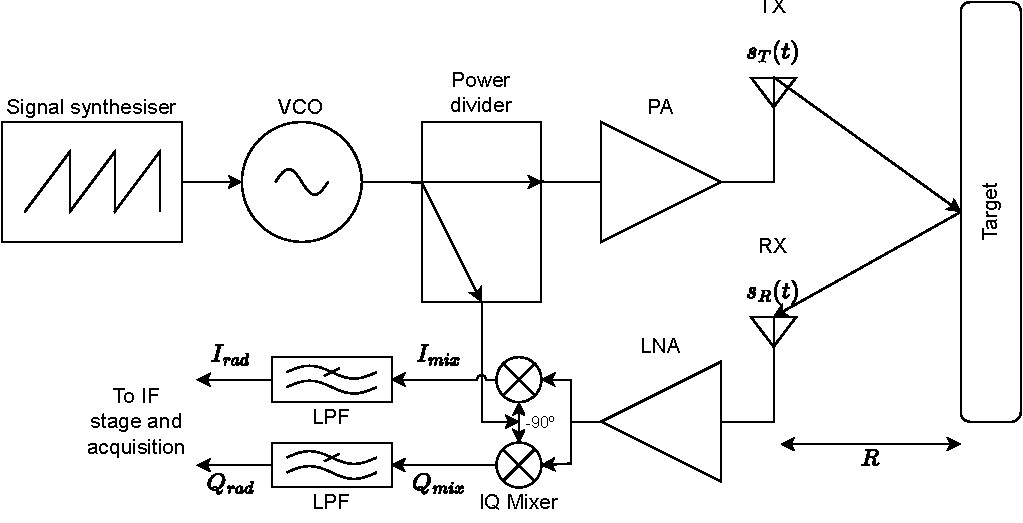
\includegraphics[width=0.7\linewidth]{CWLFM}
	\caption[Basic architecture of a CWLFM radar.]{Basic architecture of a CWLFM radar (adapted from \cite{Sardinero2022}).}
	\label{fig_cwlfm_arch}
\end{figure}

The transmitted signal is reflected by a target located at a distance $R(\tau_m)$. $\tau_m$ is the \textit{slow time} defined by \cref{eqn_slowtime} where $m$ is each transmission instant \cite{Ziemer2009}. The received signal scattered from such target is defined by equation \cref{eqn_sr} \cite{Ziemer2009,Sardinero2022} where $\sigma$ is the radar cross section (RCS) of the target and $\frac{2R(\tau_m)}{c}$ is the round trip delay. The equation assumes that the target position or movement does not change during each repetition interval $T_c$. An example of a received signal is shown in \cref{fig_cwlfm_ramps_freq}.
\begin{gather}
	\tau_m = t(m T_c); \qquad \forall m \in \mathbb{Z} \label{eqn_slowtime}\\
	s_R(t, \tau_m) = \sqrt{\sigma} \cdot \cos\left[ 2 \pi f_0 \left( t - \frac{2R(\tau_m)}{c}\right) + \pi \alpha \left( t - \frac{2R(\tau_m)}{c}\right)^2 \right] \label{eqn_sr}
\end{gather}

By beating $s_T(t)$ and $s_R(t)$ a beat signal is generated $s_b(t, \tau_m)$. The beat signal contains information in its frequency. The frequency of the beat signal (also called \textit{beat frequency}) $f_b(\tau_m)$ is proportional to the target distance $R(\tau_m)$ as shown in \cref{eqn_fb} \cite{Sardinero2022}. The beat frequency is the difference of the frequencies of the transmitted and received signals. \cref{eqn_fb} holds only at the time intervals where transmitted and received ramps are within the same period \cite{Sardinero2022}. The received signal and the manifestation of the beat frequency as the frequency difference between transmitted and received signals is depicted in \cref{fig_cwlfm_diff}.
\begin{equation} \label{eqn_fb}
	f_b(\tau_m)=\frac{2 \alpha R(\tau_m)}{c} = \frac{2 W R(\tau_m)}{c T_c}
\end{equation}

\begin{figure}[ht]
	\centering
	\subfloat[Frequency variation with time of the transmitted and received signals, where $\Delta t = \frac{2 R(\tau_m)}{c}$.]{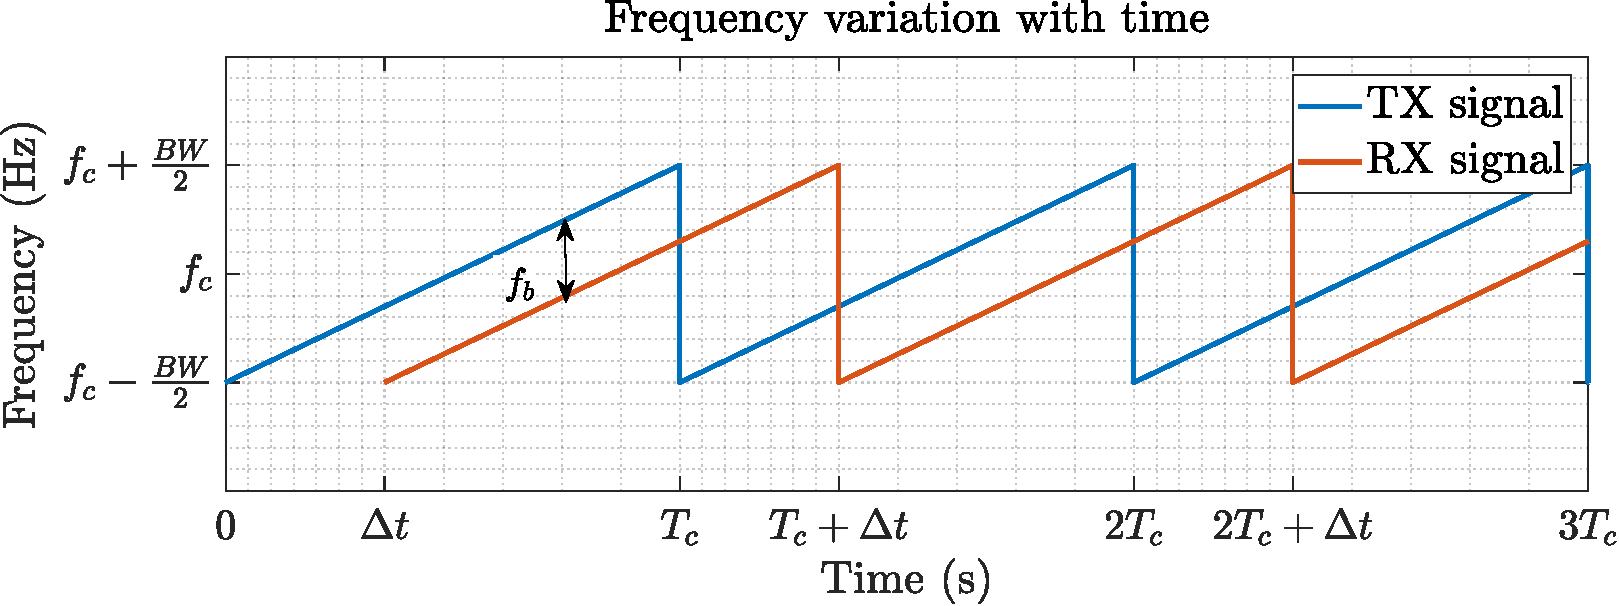
\includegraphics[width=0.8\linewidth]{cwlfm_ramps} \label{fig_cwlfm_ramps_freq}}\\
	\subfloat[Beat frequency variation with time.]{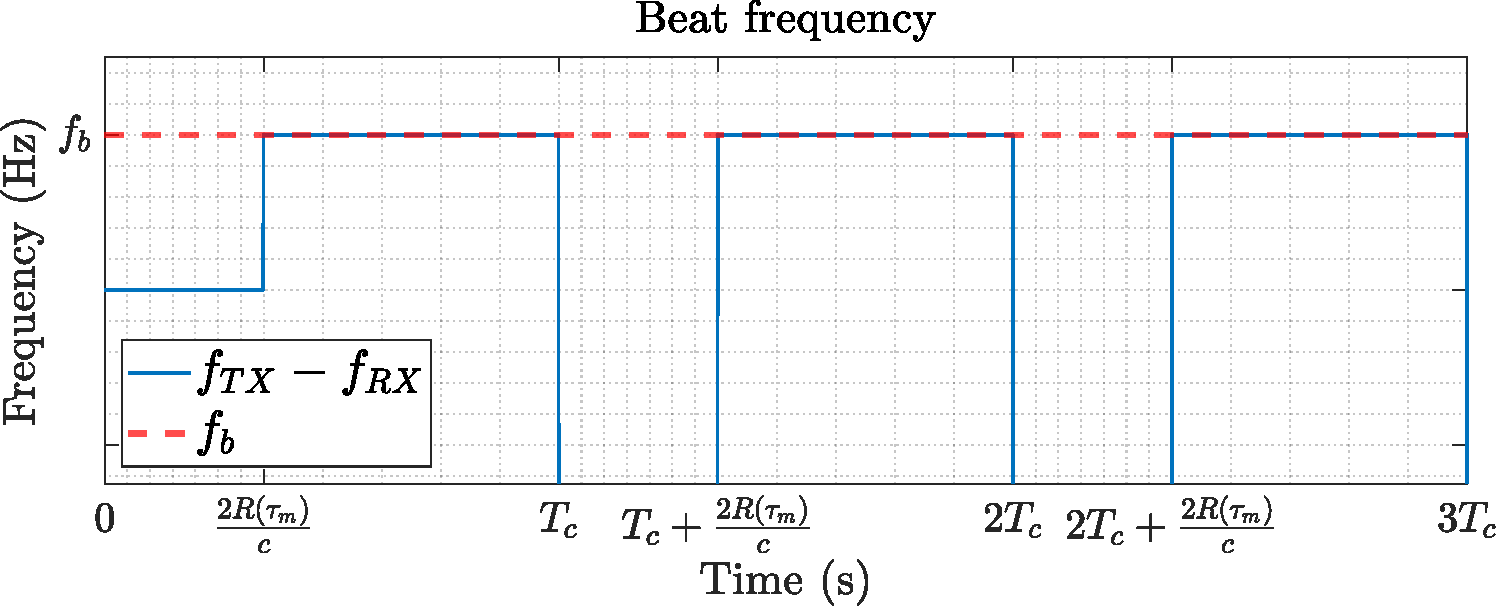
\includegraphics[width=0.8\linewidth]{cwlfm_fb} \label{fig_cwlfm_diff}}
	\caption[Beat frequency for the transmitted and received signal scattered by a target at $R(\tau_m)$ meters away from the radar. Note that the beat frequency is the difference between frequencies of transmitted an received signals at the time intervals where transmitted and received ramps are within the same period.]{Beat frequency for the transmitted and received signal scattered by a target at $R(\tau_m)$ meters away from the radar. Note that the beat frequency is the difference between frequencies of transmitted an received signals at the time intervals where transmitted and received ramps are within the same period \cite{Sardinero2022}. 		\label{fig_cwlfm_ramps}}
\end{figure}

The beat frequency is used for target location, allowing the monitorisation of several people simultaneously \cite{Antolinos2020}. The location can be found by performing the fast Fourier transform (FFT) of the beat signal. The minimum physical separation between to targets so that they can be detected independently (called \textit{range resolution}) can be obtained from \cref{eqn:range_res}, where $W$ is the swept bandwidth % and $\sigma \ge 1$ a parameter bound to FFT windowing characteristics
\cite{Sardinero2022}.
\begin{equation} \label{eqn:range_res}
	\Delta R = \frac{c}{2W} % TODO: REVISAR \Delta R = \frac{\alpha c}{2W}
\end{equation}

\label{sec:radar_op}
The resulting IF signal is digitised and processed by an analogue-to-digital converter (ADC). The sampling frequency of the ADC is important in order to avoid valuable information loss.

The Nyquist Theorem \cite{Shannon1949} establishes the relationship between the maximum frequency of the signal and the sampling frequency to avoid information loss:
\begin{equation} \label{eq:nyquist}
	2 f_{b \max} \le f_s
\end{equation}
where $f_{b \max}$ is the maximum frequency of the output signals $I_{\mathrm{rad}}$ and $Q_{\mathrm{rad}}$ in \cref{fig_cwlfm_arch}.

The maximum range of the radar $(R_{\max})$ determines the maximum frequency of the IF output signal:
\begin{equation}\label{eq:range_max}
	R_{\max} = \frac{f_{b \max} c}{2 \alpha} \implies f_{b \max} = \frac{2R_{\max} \alpha}{c}
\end{equation}
where $\alpha$ is the slope of the frequency ramp and $c$ is the speed of light.

The pulse repetition interval limits the maximum Doppler frequency ($f_{d\max}$) that can be extracted from the signal \cite{Amin2017}:
\begin{equation} \label{eq:doppler_max_tc}
	f_{d\max} = \frac{1}{2 T_c}
\end{equation}

The Doppler frequency $f_d$ is related to the radial velocity of the target $\nu_r$ as follows \cite{Richards2010}:
\begin{equation} \label{eq:doppler_max_vr}
	f_d = \frac{2 f_0 \nu_r}{c} \implies f_{d\max} = \frac{2 f_0 \nu_{r\max}}{c}
\end{equation}
where $f_0$ is the central frequency of the radar and $\nu_{r\max}$ is the maximum radial velocity of the target.

By combining \cref{eq:nyquist,eq:range_max,eqn_chirp,eq:doppler_max_tc,eq:doppler_max_vr} the following relationship is obtained:
\begin{equation} \label{eq:fs_final}
	f_s \ge \frac{16 R_{\max}W f_0 \nu_{r\max}}{c^2}
\end{equation}

To enable processing and acquisition of this signal, it is important to use hardware that meets specific requirements.

One way to obtain information from the velocity of the target is by processing the CWLFM signals in frequency and generating a Doppler-time matrix \cite{Amin2017,Richards2010}. The process of obtaining this matrix is described in \cref{fig:range_doppler_matrix}. This is extremely useful in the context of gait analysis introduced in \cref{sec:gait_methods}, as valuable information about the velocity of the extremities of the target human being can be extracted \cite{Senigagliesi2020}.

\begin{figure}[ht]
	\centering
	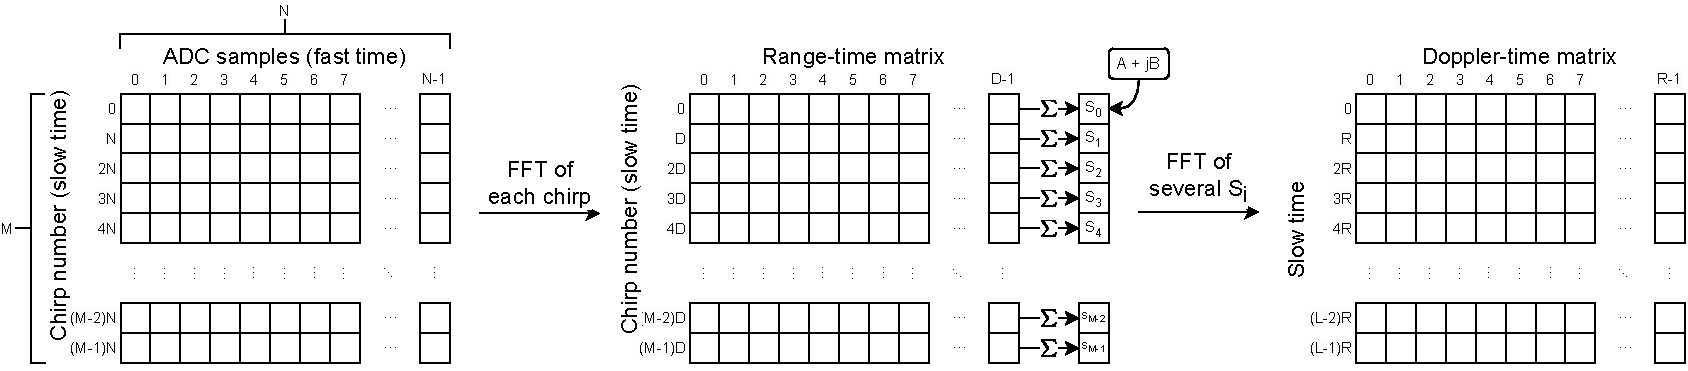
\includegraphics[width=\linewidth]{range_doppler_matrix.pdf}
	\caption{Doppler-time matrix mapping. Each ramp of the CWLFM radar signal is sampled. A FFT is computed for every ramp. Additionally the frequency components for every ramp are summed and an FFT of several sums is performed to extract the Doppler information.}
	\label{fig:range_doppler_matrix}
\end{figure}

\section{Hardware requirements for generation and processing of CWLFM signals} \label{sec:general_hw_req}
\sectionmark{Hardware requirements}

As seen in \cref{sec:radar_op}, depending on the variation and range of the magnitudes of interest to be measured, different hardware requirements must be met. In this section, they are detailed the hardware characteristics and parts of the radar system necessary to enable correct processing of the CWLFM radar signals. For the purpose of describing the necessary hardware components \cite{Richards2010}, the current CWLFM 24 GHz radar node developed at GMR-SSR \cite{Sardinero2022, Montesano2019} is used.

Based on most commercial solutions for CWLFM radars \cite{Peng2019}, the radar system integrates three main stages:
\begin{itemize}
	\item An RF stage containing the radiating elements and RF integrated circuits (IC).
	\item A radar control stage which feeds control signals to the RF board and conditions the received RF signals so as to output baseband (intermediate frequency, IF) signals.
	\item An acquisition stage featuring an analogue-to-digital converter (ADC) responsible for the digitisation of the CWLFM signals for posterior processing and/or transmission to extract useful information.
\end{itemize}
 In the current system, the control board conditions the signals from the RF stage and outputs baseband signals which are driven directly to the acquisition stage. A diagram showing the elements present in the currently developed radar node is shown in \cref{fig:current_system}.

\begin{figure}[ht]
	\centering
	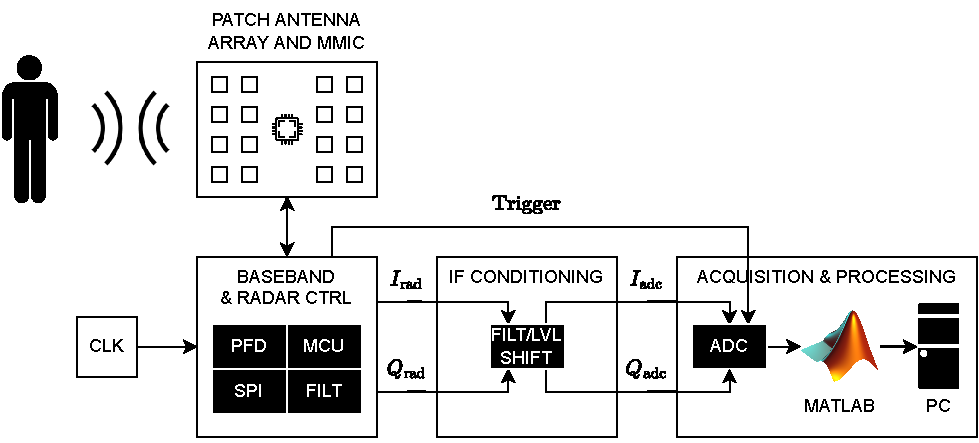
\includegraphics[width=\linewidth]{complete_sys_pc.pdf}
	\caption{Overview of the full radar system components of the currently developed 24 GHz CWLFM radar with corresponding inputs and outputs. Conditioned baseband signals are denoted as $I_{\mathrm{rad}}$ and $Q_{\mathrm{rad}}$. Signals at the input of the acquisition stage are denoted as $I_{\mathrm{adc}}$ and $Q_{\mathrm{adc}}$. A trigger signal coming from the radar control board is denoted as \textit{Trig}. In the current system, the conditioned signals output from the radar control board are directly sampled by an external ADC and $I_{\mathrm{rad}} = I_{\mathrm{adc}},Q_{\mathrm{rad}} = Q_{\mathrm{adc}}$. \label{fig:current_system}}
\end{figure}

\subsection{RF stage} \label{sec:rf_board_general}

A printed circuit board (PCB) contains the antennas and the radar MMIC. This PCB contains two patch array antennas. One antenna is used for the signal transmission while the other is used for the reception of the rebound signal from the target. The antennas are connected to a monolithic microwave integrated circuit (MMIC) from Silicon Radar model TRX-024-046 \cite{SR2021} which provides an output RF signal for transmission and two intermediate frequency (IF) signals in I and Q format from the reception. It is important that the field of view of the antenna is large enough to contain the target. The high-level diagram of the MMIC is shown in \cref{fig:block_mmic_general}.

\begin{figure}[ht]
	\centering
	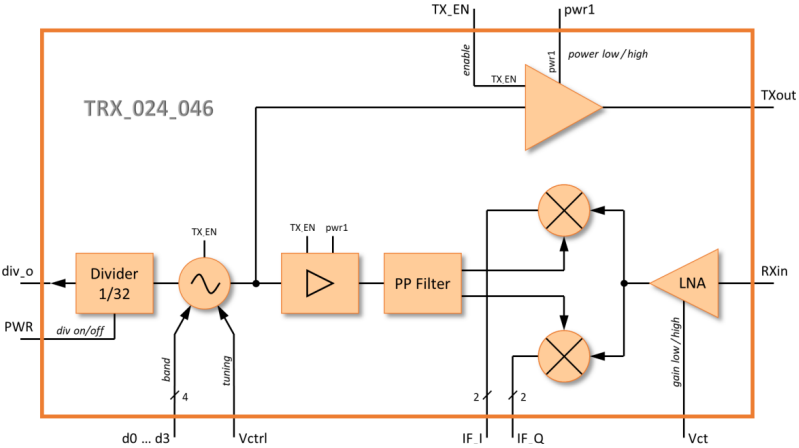
\includegraphics[width=0.7\linewidth]{block_mmic_datasheet.png}
	\caption[High-level diagram of the TRX-024-046 MMIC. The tuning voltage is controlled by the DC level on the \textit{Vctrl} pin and the bandwidth is selected with the \textit{d0...d3} pins. The resulting beating signals are output in the \textit{IF\_I} and \textit{IF\_Q} pins. It is important to note that each pair of IF signals is in differential form.]{High-level diagram of the TRX-024-046 MMIC. The tuning voltage is controlled by the DC level on the \textit{Vctrl} pin and the bandwidth is selected with the \textit{d0...d3} pins. The resulting beating signals are output in the \textit{IF\_I} and \textit{IF\_Q} pins. It is important to note that each pair of IF signals is in differential form \cite{SR2021}. \label{fig:block_mmic_general}}
\end{figure}

The signal provided to the transmission antenna is produced by a voltage controlled oscillator, whose bandwidth is configurable and the tuning is provided by a voltage control pin \textit{Vctrl} \cite{SR2021}. This control voltage is generated in an adjacent radar control board described in \cref{sec:baseband_general} connected to this PCB through pinhole connectors. This PCB is manufactured in FR4 dielectric material for the core and is part of the SiRadar EvalKit Easy evaluation kit from Silicon Radar \cite{SR2021eval}. An image of the aforementioned PCB with the antennas and MMIC is shown in  \cref{fig:rf_board_general}.

\begin{figure}[ht]
	\centering
	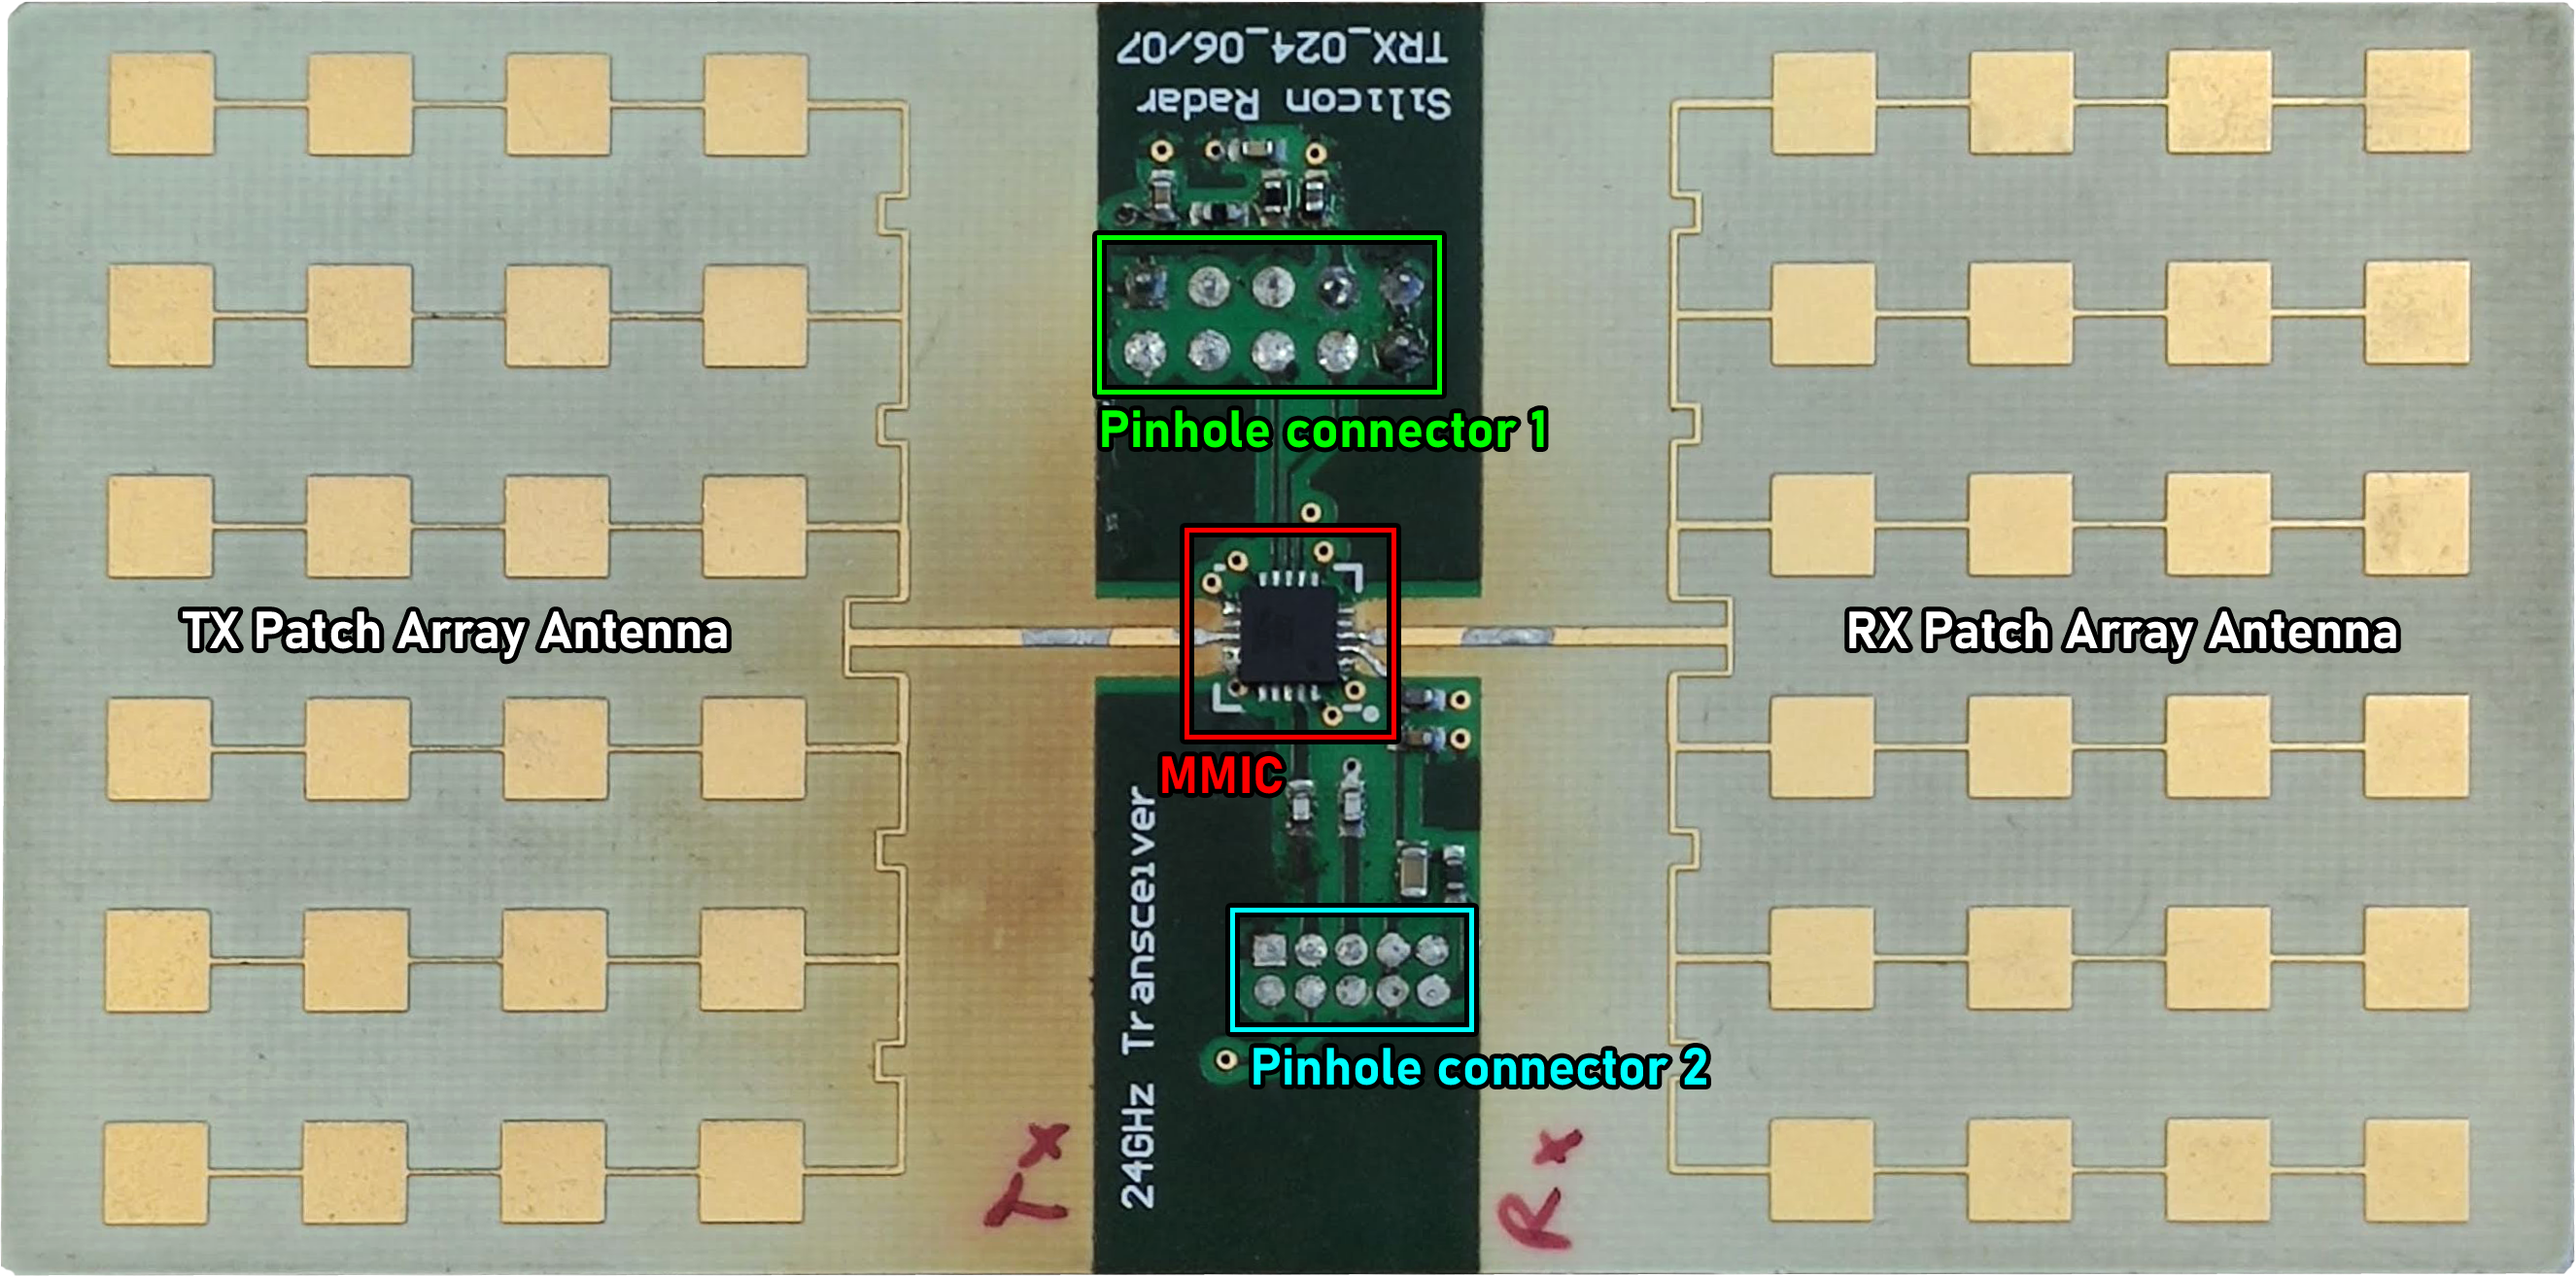
\includegraphics[width=0.7\linewidth]{radar_antenna_mmic.png}
	\caption{Patch antenna and MMIC PCB used in the PCB radar node. The different components are outlined in the image. \label{fig:rf_board_general}}
\end{figure}

\subsection{Radar control stage} \label{sec:baseband_general}

The radar control stage provides the MMIC with the \textit{Vctrl} signal in order to generate the CWLFM ramp signals based on a predefined chirp time and frequency. Additionally, the radar control stage conditions the IF signals coming from the MMIC. The connection with the RF board is via two pinhole connectors.

This signal is provided by a frequency synthesiser based on a phase-frequency detector (PFD), a precision charge pump (CP) and a reference divider. These elements come bundled in a phase-locked loop (PLL) architecture \cite{Sardinero2022}.

The PFD used in the radar control PCB developed at GMR-SSR is from Analog Devices, model ADF4159 \cite{TexasInstrumentsADF}. The PFD allows configuring parameters such as the bandwidth swept, the ramp or chirp time and the clock source selection through a serial parallel interface (SPI) connection by writing to some specific registers of the PFD integrated circuit (IC) \cite{Sardinero2022, TexasInstrumentsADF}. Therefore, the board also integrates a microcontroller unit (MCU) that is programmed to write to the registers as described in \cite{Sardinero2022}. A detailed description of the PLL architecture of the VCO can be found in \cite[p.~92-94]{Sardinero2022}.
For every ramp of the signal, trigger signals are output in the \textit{Trig} output. The trigger signals are described in \cref{sec:trigger_signal_characterisation}.

Finally, the IF signals output by the RF stage are amplified and conditioned to provide a sufficient voltage excursion to enable processing \cite{Sardinero2022}. Therefore amplifying and filtering components are present in this stage. These components provide a gain of \SI{14}{dB} and a bandwidth of \SI{3}{\mega\hertz}. The amplifying and filtering components are described in \cite[p.~83-87]{Sardinero2022}.
These signals output by the radar control stage are denominated $I_\mathrm{rad}$ and $Q_\mathrm{rad}$, respectively.

The radar control PCB is manufactured in FR4 dielectric material for the core by the manufacturer Eurocircuits. An image of the manufactured radar control board is found in \cref{fig:baseband_board_general}.

\begin{figure}[htb]
	\centering
	\subfloat[Bottom view]{\includegraphics[width=0.41\linewidth]{img/radar_pcb_bot.png} \label{fig:baseband_board_general_bot}}
	\subfloat[Top view]{\includegraphics[width=0.4\linewidth]{img/radar_pcb_top.png} \label{fig:baseband_board_general_top}}
	\caption{Top and bottom views of a manufactured PCB layout of the radar control stage. The elements of this board are outlined by coloured rectangles. Some components are not used in the current radar node design so they are removed, these elements are outlined by grey rectangles. \label{fig:baseband_board_general}}
\end{figure}

%\subsection{Intermediate frequency (IF) stage}
%
%Signals output from the radar control board have a predetermined voltage range and frequency characteristics. Most embedded ADCs have an input range covering only positive voltage values, differing from the input signal peak-to-peak voltage excursion. The I and Q signals output from the radar control board must be conditioned to the ADC voltage input range and the output impedance must be matched to the ADC input impedance.
%
%In many instances, the output signals from the radar control board lack DC level and the radar control stage voltage excursion is not adapted to the ADC voltage range, allowing high discretization errors. Moreover, some MMICs \cite{Antolinos2020} output baseband signals in a differential format. For single-ended ADCs, the signals must be converted to single-ended format.
%% TODO: cambiar cita de elias a una buena
%
%Nonetheless, this stage is not necessary provided that the ADC input voltage range can be adjusted and fitted to the baseband signals voltage excursion and the output configuration matches the input configuration of the ADC.
%
%Should it be necessary to condition the signal, an intermediate frequency (IF) stage is used. The IF stage provides gain and DC shifting to the input signals for correct digitisation. To that effect, the IF stage must have the following capabilities:
%\begin{itemize}
%	\item Conversion from differential to single-ended signal configurations (bypassable)
%	\item Linear, low-noise amplification, filtering and DC shifting
%\end{itemize}
%
%A high-level overview of the architecture for this stage is shown in \cref{fig:if_general}. This stage can be laid out in a separate board to prioritise modularity or integrated with other stages in a single board to favour compactness and power efficiency.
%
%\begin{figure}[ht]
%	\centering
%	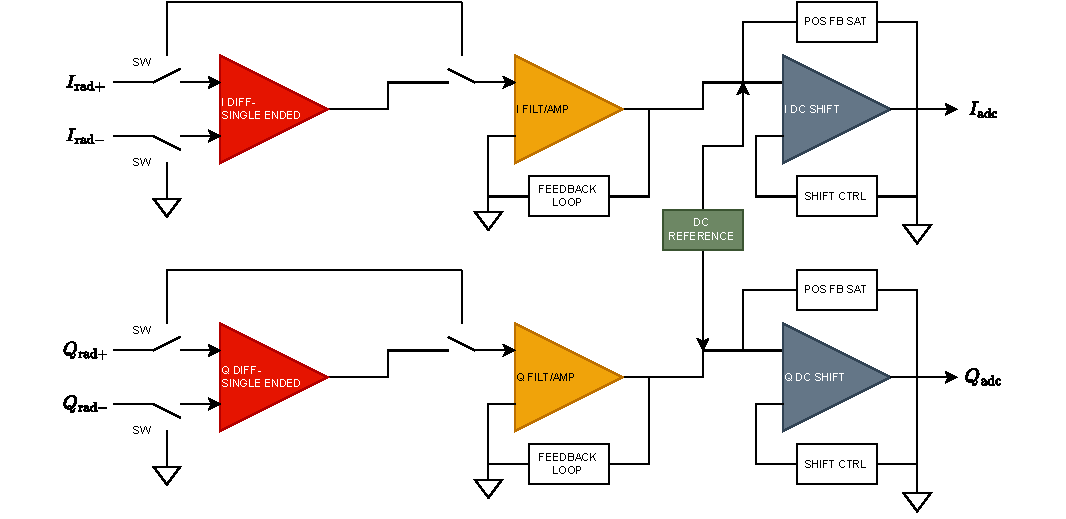
\includegraphics[width=\linewidth]{if_stage_diagram.pdf}
%	\caption{High-level architecture of the intermediate frequency (IF) stage for signal conditioning and impedance matching \label{fig:if_general}}
%\end{figure}

\subsection{Acquisition stage}

In the current design, the IF signals from the radar control board (namely, $I_\mathrm{rad}$ and $Q_\mathrm{rad}$) are driven directly to the acquisition stage. Conversion of the filtered and conditioned signals from the analogue domain to a digital representation is carried out in this stage. The current implementation features an acquisition stage composed of an ADC connected to a PC, which follows the current commercial and state-of-the-art implementations \cite{Antolinos2020,Biase2020,Zanardi2021,Seifert2019, Iyer2022, Amin2017}. This setup allows for post-processing the captured signals on the PC.

To subsequently achieve a correct sampling of the signals, the ADC must be able to sample at a rate higher than the minimum sample rate $f_s$ as per \cref{eq:fs_final}, which is dependant of the Nyquist criteria outlined in \cref{eq:nyquist} and the Doppler range-frequency characteristic shown in \cref{eq:doppler_max_vr}. These characteristics vary depending on the application, for instance, they rely on the maximum Doppler velocity to be measured. Ensuring correct acquisition in a wide variety of scenarios can only be achieved by selecting an ADC with a sufficiently high $f_{s_{\max}}$. The implementation of the radar node available at GMR-SSR makes use of the ADLINK Technologies PCI-9846 ADC card \cite{ADLINKTechnologies2010, Sardinero2022}.

\cref{fig:adc_general} shows a high-level diagram describing the hardware present in the acquisition stage of the currently developed radar node. Signals from the radar control stage are connected directly to the ADC and sampled. Trigger signals from the radar control board are also input to the ADC to determine the sampling instants. The processing pipeline features a digitiser card connected to a PC via a high-speed Peripheral Component Interconnect (PCI) port. The ADC card is instructed by a control program written in MATLAB \cite{Antolinos2020, Sardinero2022} to sample for a predetermined amount of time at a particular sampling frequency. After collecting the samples and storing them on the on-board memory of the ADC, they are transferred to the random access memory (RAM) of the computer to be accessed by a digital signal processing (DSP) software also written in MATLAB \cite{Antolinos2020, Sardinero2022}. It is important to note that the sampling and processing is done in a deferred way, as the DSP takes place after the measurement capture process finishes \cite[p.~43-44]{ADLINKTechnologies2010}.

\begin{figure}[ht]
	\centering
	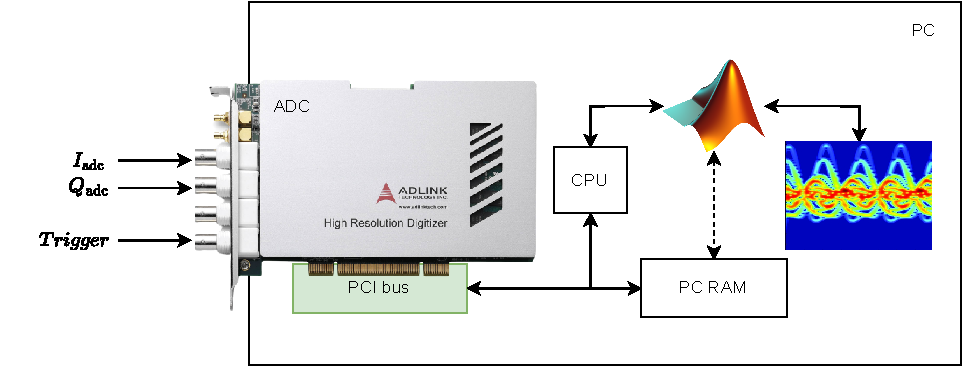
\includegraphics[width=0.7\linewidth]{adc_stage_pc_diagram.pdf}
	\caption{High-level architecture of the acquisition stage for signal digitisation. \label{fig:adc_general}}
\end{figure}


\section{Hardware cost} \label{sec:hw_cost}

The different stages described in \cref{sec:general_hw_req} are composed of a set of materials and hardware components that form the complete system of one radar node. It is of interest to analyse the final cost of manufacturing one radar node.

State-of-the-art commercial implementations follow the requirements outlined in \cref{sec:general_hw_req}. A specific implementation has been developed at GMR-SSR that features the stages present on a CWLFM radar node \cite{Sardinero2022}. For this implementation, the cost per unit of a single radar node has been analysed at the time of writing. A summarised overview of the cost per part of the system is shown in \cref{tab:cost_stages}. The detailed cost per component for a single node is outlined in \cref{app:detailed_cost_current}.

Firstly, it can be seen that the radar control stage contributes minimally to the overall cost, despite being somewhat expensive derived from the cost of the RF components. Nonetheless, the most expensive stage by far is the acquisition stage. In fact, this stage contributes to almost the entirety of the cost of the system. Conclusively, a radar node costing almost as much as the cost of the its acquisition stage is not a figure of merit of the system.

\begin{table}
	\centering
	\begin{tblr}{
			width = \linewidth,
			colspec = {X[3,l]
				X[2,si={table-format=3.2,table-number-alignment=right},r]
				X[3,si={table-format=3.2,table-number-alignment=right},r]},
			row{1,Z} = {font=\bfseries},
		}
		\toprule
		{{{Stage}}} & {{{Subtotal (€)}}} & {{{Contribution to total cost (\%)}}}\\
		\midrule
		Radar control stage & 389.13 & 6.75 \\
		Acquisition stage & 5380.00 & 93.25 \\
		\hspace{0.2cm} └─ PC & 950.00 & 16.47 \\
		\hspace{0.2cm} └─ MATLAB License & 800.00 & 13.87\\
		\hspace{0.2cm} └─ ADC (ADLINK PCI-9846) & 3630.00 & 62.92 \\
		\midrule
		Total cost & 5747.79  & 100.00 \\
		\bottomrule
	\end{tblr}
	\caption{Cost breakdown of a radar node following the general design.}
	\label{tab:cost_stages}
\end{table}

To understand the high cost of the acquisition stage, it is of interest to study the parts included in the general design of this stage \cite{Sardinero2022}. \cref{tab:cost_stages} also details the cost of the different parts comprising the acquisition stage of the current design. It is shown that the ADC itself assumes more than half the cost of a single radar node. Additionally, other high costs of the stage cannot be neglected. Those costs are related with the equipment and software necessary to interface with ADC. This is currently achieved with a PC executing MATLAB \cite{Sardinero2022, Antolinos2020}. Thus, a sufficiently fast PC and a MATLAB license are required as well.

For the objective of developing multi-static radar networks, a high cost per node entails difficulties in scaling up the number of nodes to be manufactured and integrated into a system. Furthermore, the need to use a PC to obtain and process the samples poses a problem for the portability, energy efficiency and compactness of the nodes, making it difficult to integrate them in closed spaces.
In conclusion, the current state-of-the-art acquisition and processing stage and pipeline severely increases the cost of the radar nodes. In the context of the use of radar networks for gait analysis, radar nodes must be cost-effective and compact.